 \documentclass[12pt]{article}

% Include packages for mathematical symbols, figures, floating elements, and code listing
\usepackage{amsmath, amssymb, amsfonts, amsthm}
\usepackage{graphicx}  % Allows for importing figures
\usepackage{float}     % For better control of figure/table placement
\usepackage{booktabs}  % Professional table formatting
\usepackage{verbatim}  % For block comments
\usepackage{color}     % Allows for color customization
\usepackage{listings}  % For code listing
\usepackage{hyperref}  % For hyperlinks
\usepackage{placeins}  % Prevents floats from moving past a \FloatBarrier

% Define custom colors for code listings
\definecolor{dkgreen}{rgb}{0,0.6,0}
\definecolor{gray}{rgb}{0.5,0.5,0.5}
\definecolor{mauve}{rgb}{0.58,0,0.82}

% Configure the listings package for Python code
\lstset{
  frame=tb,
  language=Python,
  aboveskip=3mm,
  belowskip=3mm,
  showstringspaces=false,
  columns=flexible,
  basicstyle={\small\ttfamily},
  numbers=left,
  numberstyle=\tiny\color{gray},
  keywordstyle=\color{blue},
  commentstyle=\color{dkgreen},
  stringstyle=\color{mauve},
  breaklines=true,
  breakatwhitespace=true,
  tabsize=3
}

% Custom command for table input
\makeatletter
\def\expinput#1{\@@input#1 }
\makeatother

% Title and author information
\title{HW \#4 \\ Math/CS 471, Fall 2024}
\author{Steven Zuñiga}
\date{November 4, 2024}

\begin{document}

% Display title
\maketitle
\newpage

\section{Introduction}
Finite difference methods are widely used for numerical solutions of partial differential equations (PDEs). This report investigates a 2D finite difference scheme for computing numerical derivatives on a unit domain, as well as its parallel implementation and performance evaluation on the CARC supercomputing platform.

\section{Problem Description}
The problem domain is the unit square \(\Omega = [0, 1] \times [0, 1]\), where the function \(u(x, y)\) is defined as:
\[
u(x, y) = \cos((x+1)^{1/3} + (y+1)^{1/3}) + \sin((x+1)^{1/3} + (y+1)^{1/3}).
\]
Dirichlet boundary conditions \(g(x, y)\) are defined as:
\[
g(x, y) = u(x, y) \quad \text{for } (x, y) \in \partial \Omega.
\]

\section{Task 1: Serial Implementation and Error Analysis}
\subsection{Methodology}
The finite difference stencil used for approximating the second derivatives is:
\[
\frac{1}{h^2} \begin{bmatrix} 0 & 1 & 0 \\ 1 & -4 & 1 \\ 0 & 1 & 0 \end{bmatrix}
\]
This was implemented using the provided `poisson.py` file, creating a CSR matrix for efficient calculations.

\subsection{Analysis of CSR Matrix Rows}
For a grid size of \( n \times n \), we analyzed specific matrix rows from the CSR representation of the finite difference stencil to understand how different types of points (corner, domain wall, interior) are represented. The following matrix rows were printed from the terminal output:

\begin{verbatim}
Matrix row for corner point (0, 0):
Data: [-4.  1.  1.]
Indices: [0 1 5]

Matrix row for edge point (0, 1):
Data: [ 1. -4.  1.  1.]
Indices: [0 1 2 6]

Matrix row for interior point (1, 1):
Data: [ 1.  1. -4.  1.  1.]
Indices: [ 1  5  6  7 11]
\end{verbatim}

\subsection{Explanation of Differences}
\begin{itemize}
    \item \textbf{Corner Point (0, 0)}: This matrix row corresponds to a corner of the grid. It only has three non-zero entries, reflecting the contributions from the central point and its two neighbors (right and below). This is due to fewer adjacent grid points compared to interior points.
    \item \textbf{Domain Wall Point (0, 1)}: This row represents a point on the top boundary but not a corner. It has four non-zero entries, accounting for contributions from the left, right, below, and the central point itself. The presence of an additional neighboring point compared to the corner point explains the extra non-zero value.
    \item \textbf{Interior Point (1, 1)}: This row corresponds to a point within the grid (not on the boundary). It has five non-zero entries, indicating contributions from all four surrounding neighbors (left, right, above, below) and the central point. This full set of adjacent points results in more non-zero entries compared to edge or corner points.
\end{itemize}

\subsection{Interpretation}
The differences between these rows illustrate how boundary conditions and the finite difference stencil shape the matrix's sparsity pattern. Corner points have fewer connections due to being adjacent to only two grid points, edge points have slightly more connections, and interior points have the most due to their central placement within the grid.


\section{Results}
\subsection{Convergence Analysis}
We computed the L2 norm of the error between the exact and numerical derivatives, defined as:
\[
\|e\|_{L2} = \left( \int_{\Omega} \left(\frac{\partial^2 u}{\partial x^2} \Big|_{\text{approx}} - \frac{\partial^2 u}{\partial x^2} \Big|_{\text{exact}} + \frac{\partial^2 u}{\partial y^2} \Big|_{\text{approx}} - \frac{\partial^2 u}{\partial y^2} \Big|_{\text{exact}} \right)^2 \, dx \, dy \right)^{1/2}.
\]



\begin{figure}[h!]
\centering
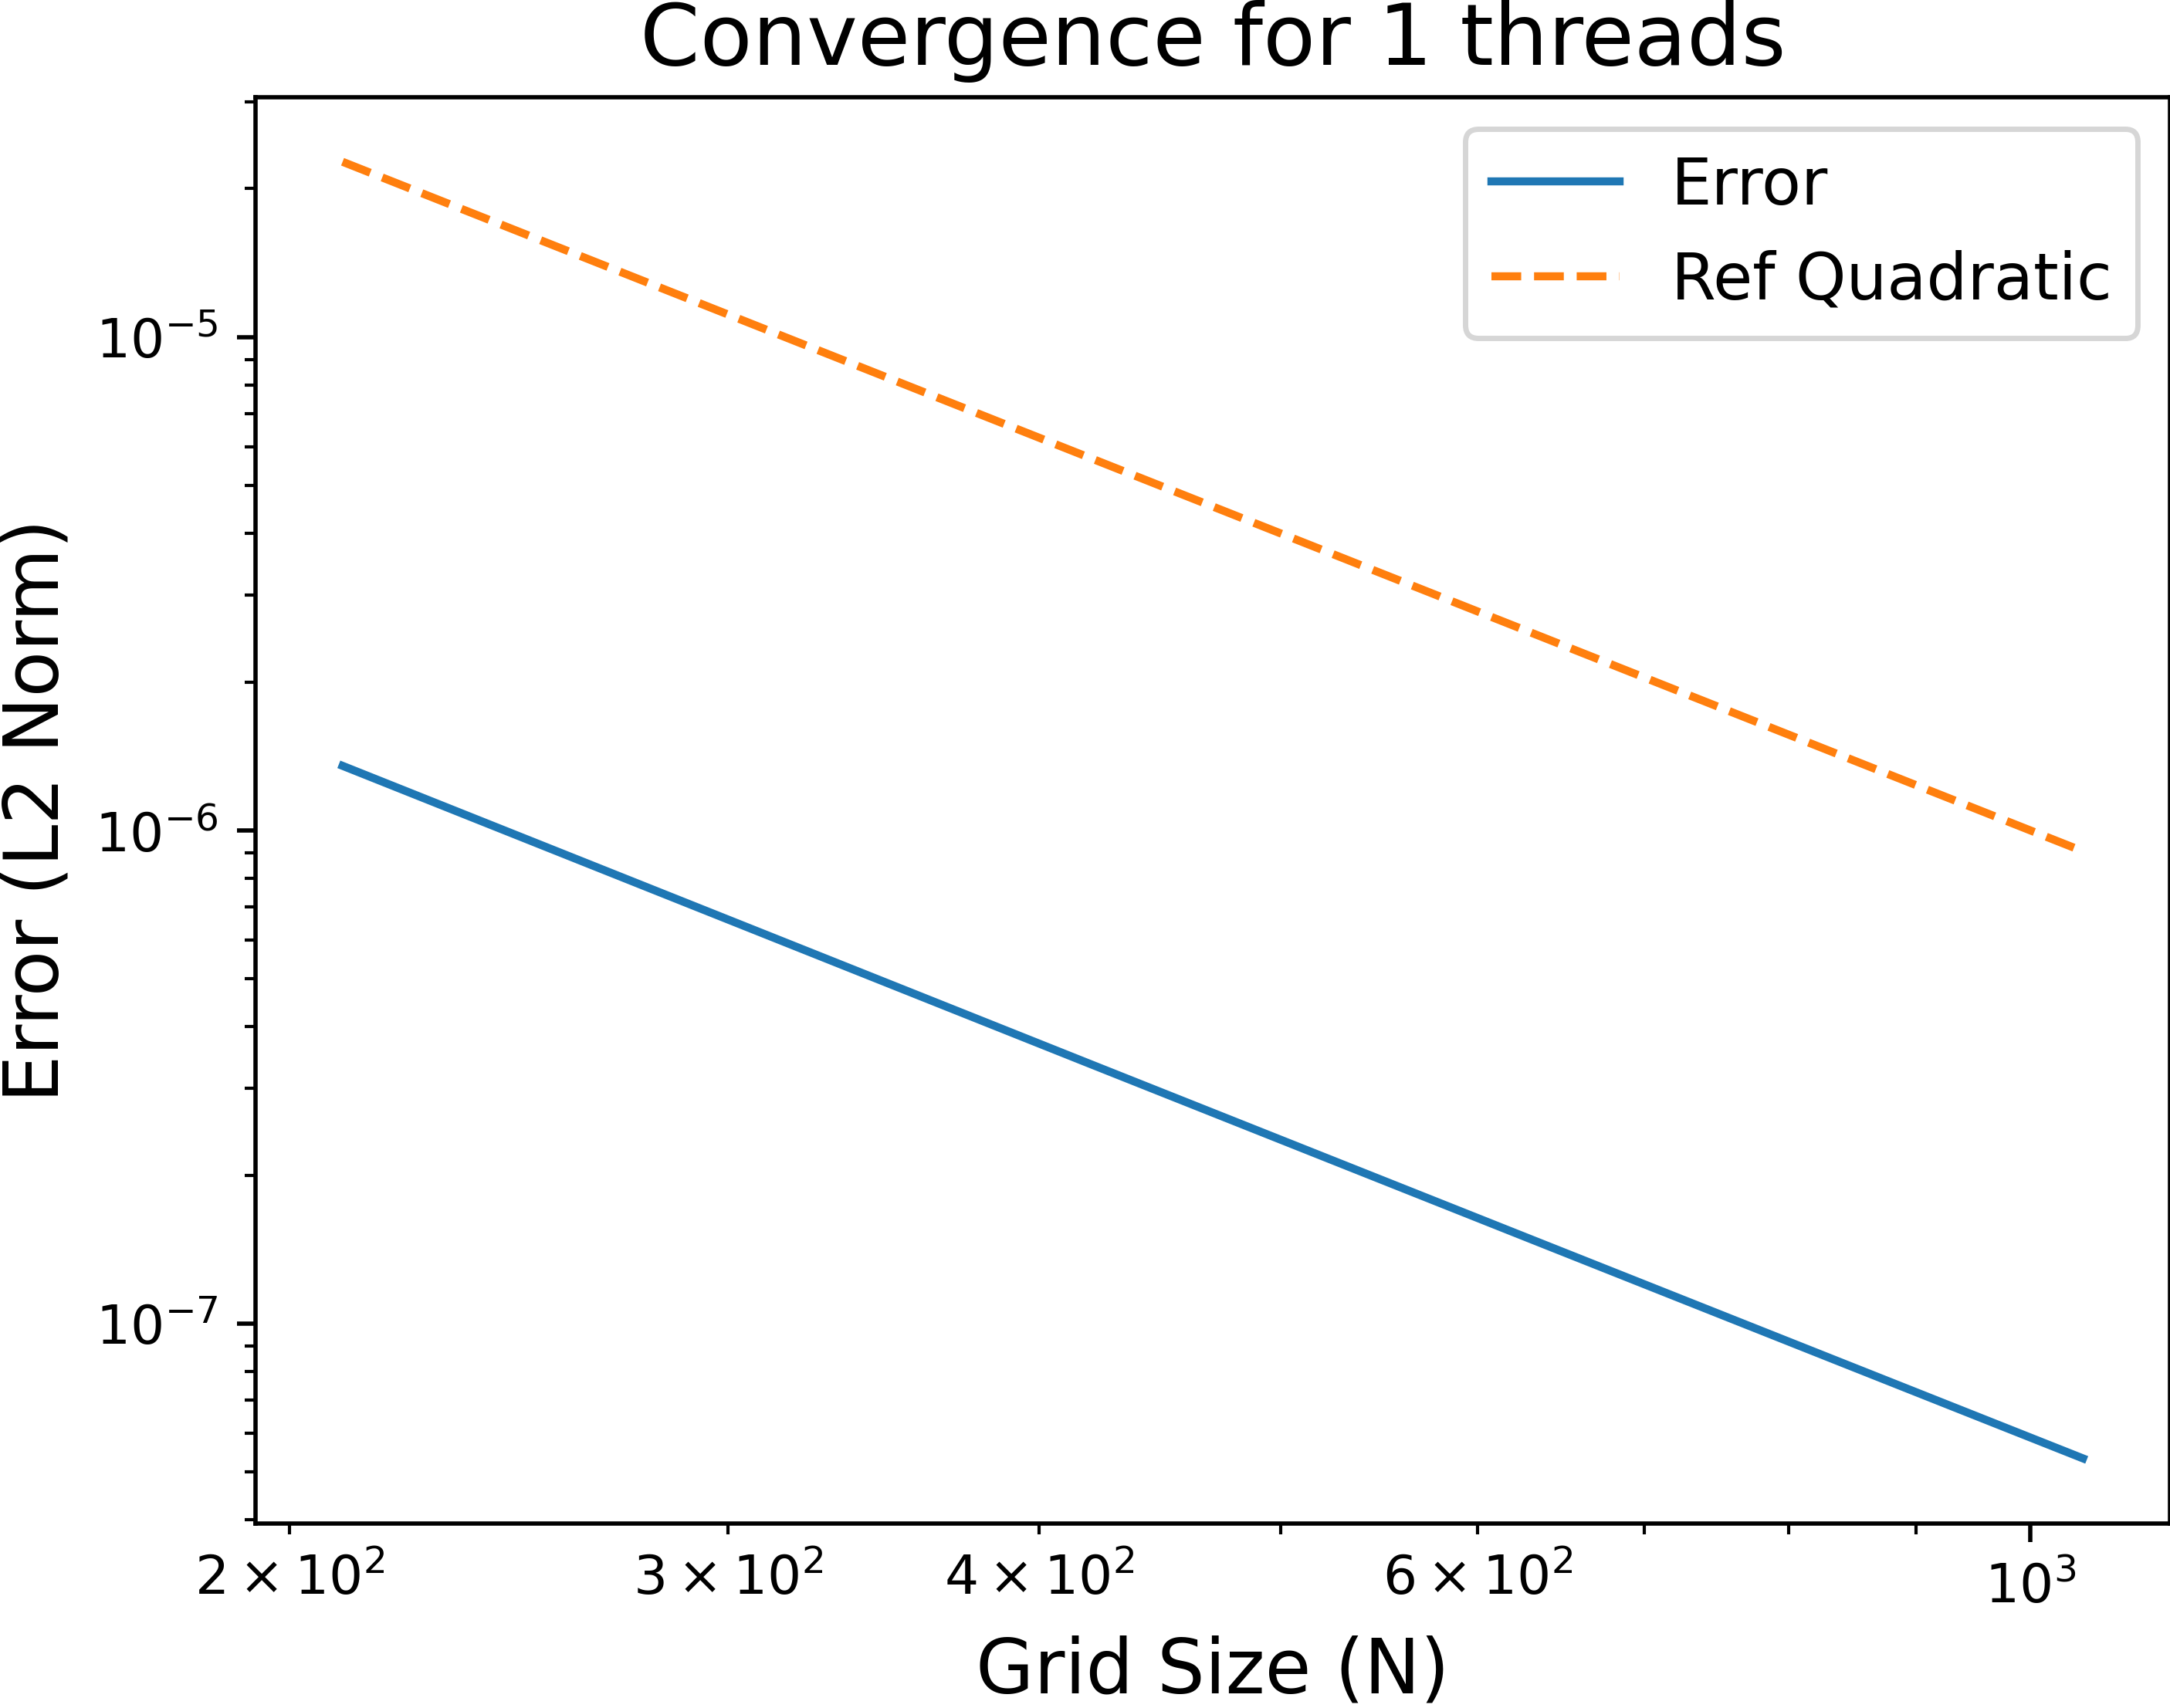
\includegraphics[width=0.5\textwidth]{/Users/stevenzuniga/Desktop/HPC/finite-difference-threading/report/error_1threadLocal.png}
\caption{Log-log plot of error vs. grid size for the serial implementation.}
\label{fig:error_serial}
\end{figure}
\FloatBarrier


The plot in Figure \ref{fig:error_serial} indicates that the numerical solution converges quadratically, consistent with the expected second-order accuracy of the finite difference method.



\FloatBarrier

%%
%Task 2
%%
\section{Task 2: Parallel Implementation and Performance Analysis}


\subsection{Timing Analysis}
Performance metrics were collected both on a local machine and the CARC computing platform.

These preliminary metrics performed locally on multiple thread counts demonstrate performance increase. This is more notably observed at three thread counts where we are able to see a noticeable increase.
The computations being observed in Table \ref{tab:local_timings} and plotted in Figure \ref{fig:timing_plots}.

\begin{table}[h!]
\centering
\begin{tabular}{|c|c|c|c|}
\hline
	Timing (s) & 	1 Thread & 	2 Threads & 	3 Threads \\ \hline
	Timing 1 & 8.5668e-03 & 8.2240e-03 & 8.0276e-03 \\ \hline
	Timing 2 & 3.6757e-02 & 3.7280e-02 & 3.4571e-02 \\ \hline
	Timing 3 & 1.0515e-01 & 1.1006e-01 & 8.9323e-02 \\ \hline
	Timing 4 & 1.9577e-01 & 2.0168e-01 & 1.7296e-01 \\ \hline
	Timing 5 & 2.9620e-01 & 3.1055e-01 & 2.7161e-01 \\ \hline
\end{tabular}
\caption{Local machine timings for different thread counts}
\label{tab:local_timings}
\end{table}

\begin{figure}[h!]
\centering
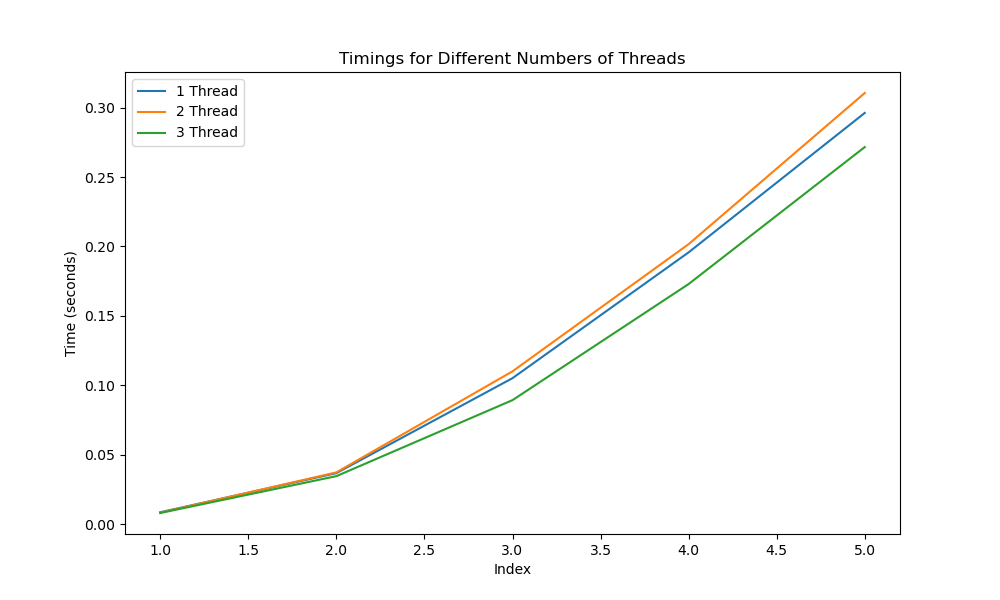
\includegraphics[width=1.2\textwidth]{/Users/stevenzuniga/Desktop/HPC/finite-difference-threading/report/timings_plot.png}
\caption{Parallel efficiency vs. number of threads.}
\label{fig:timing_plots}
\end{figure}

\section{Parallel Validation}

To validate that the parallel code produces the same results as the serial code, we analyzed the error for thread counts ranging from 1 to 3. The log-log plots of the error for each thread count are shown below.

%1-thread
\begin{figure}[H]
\centering
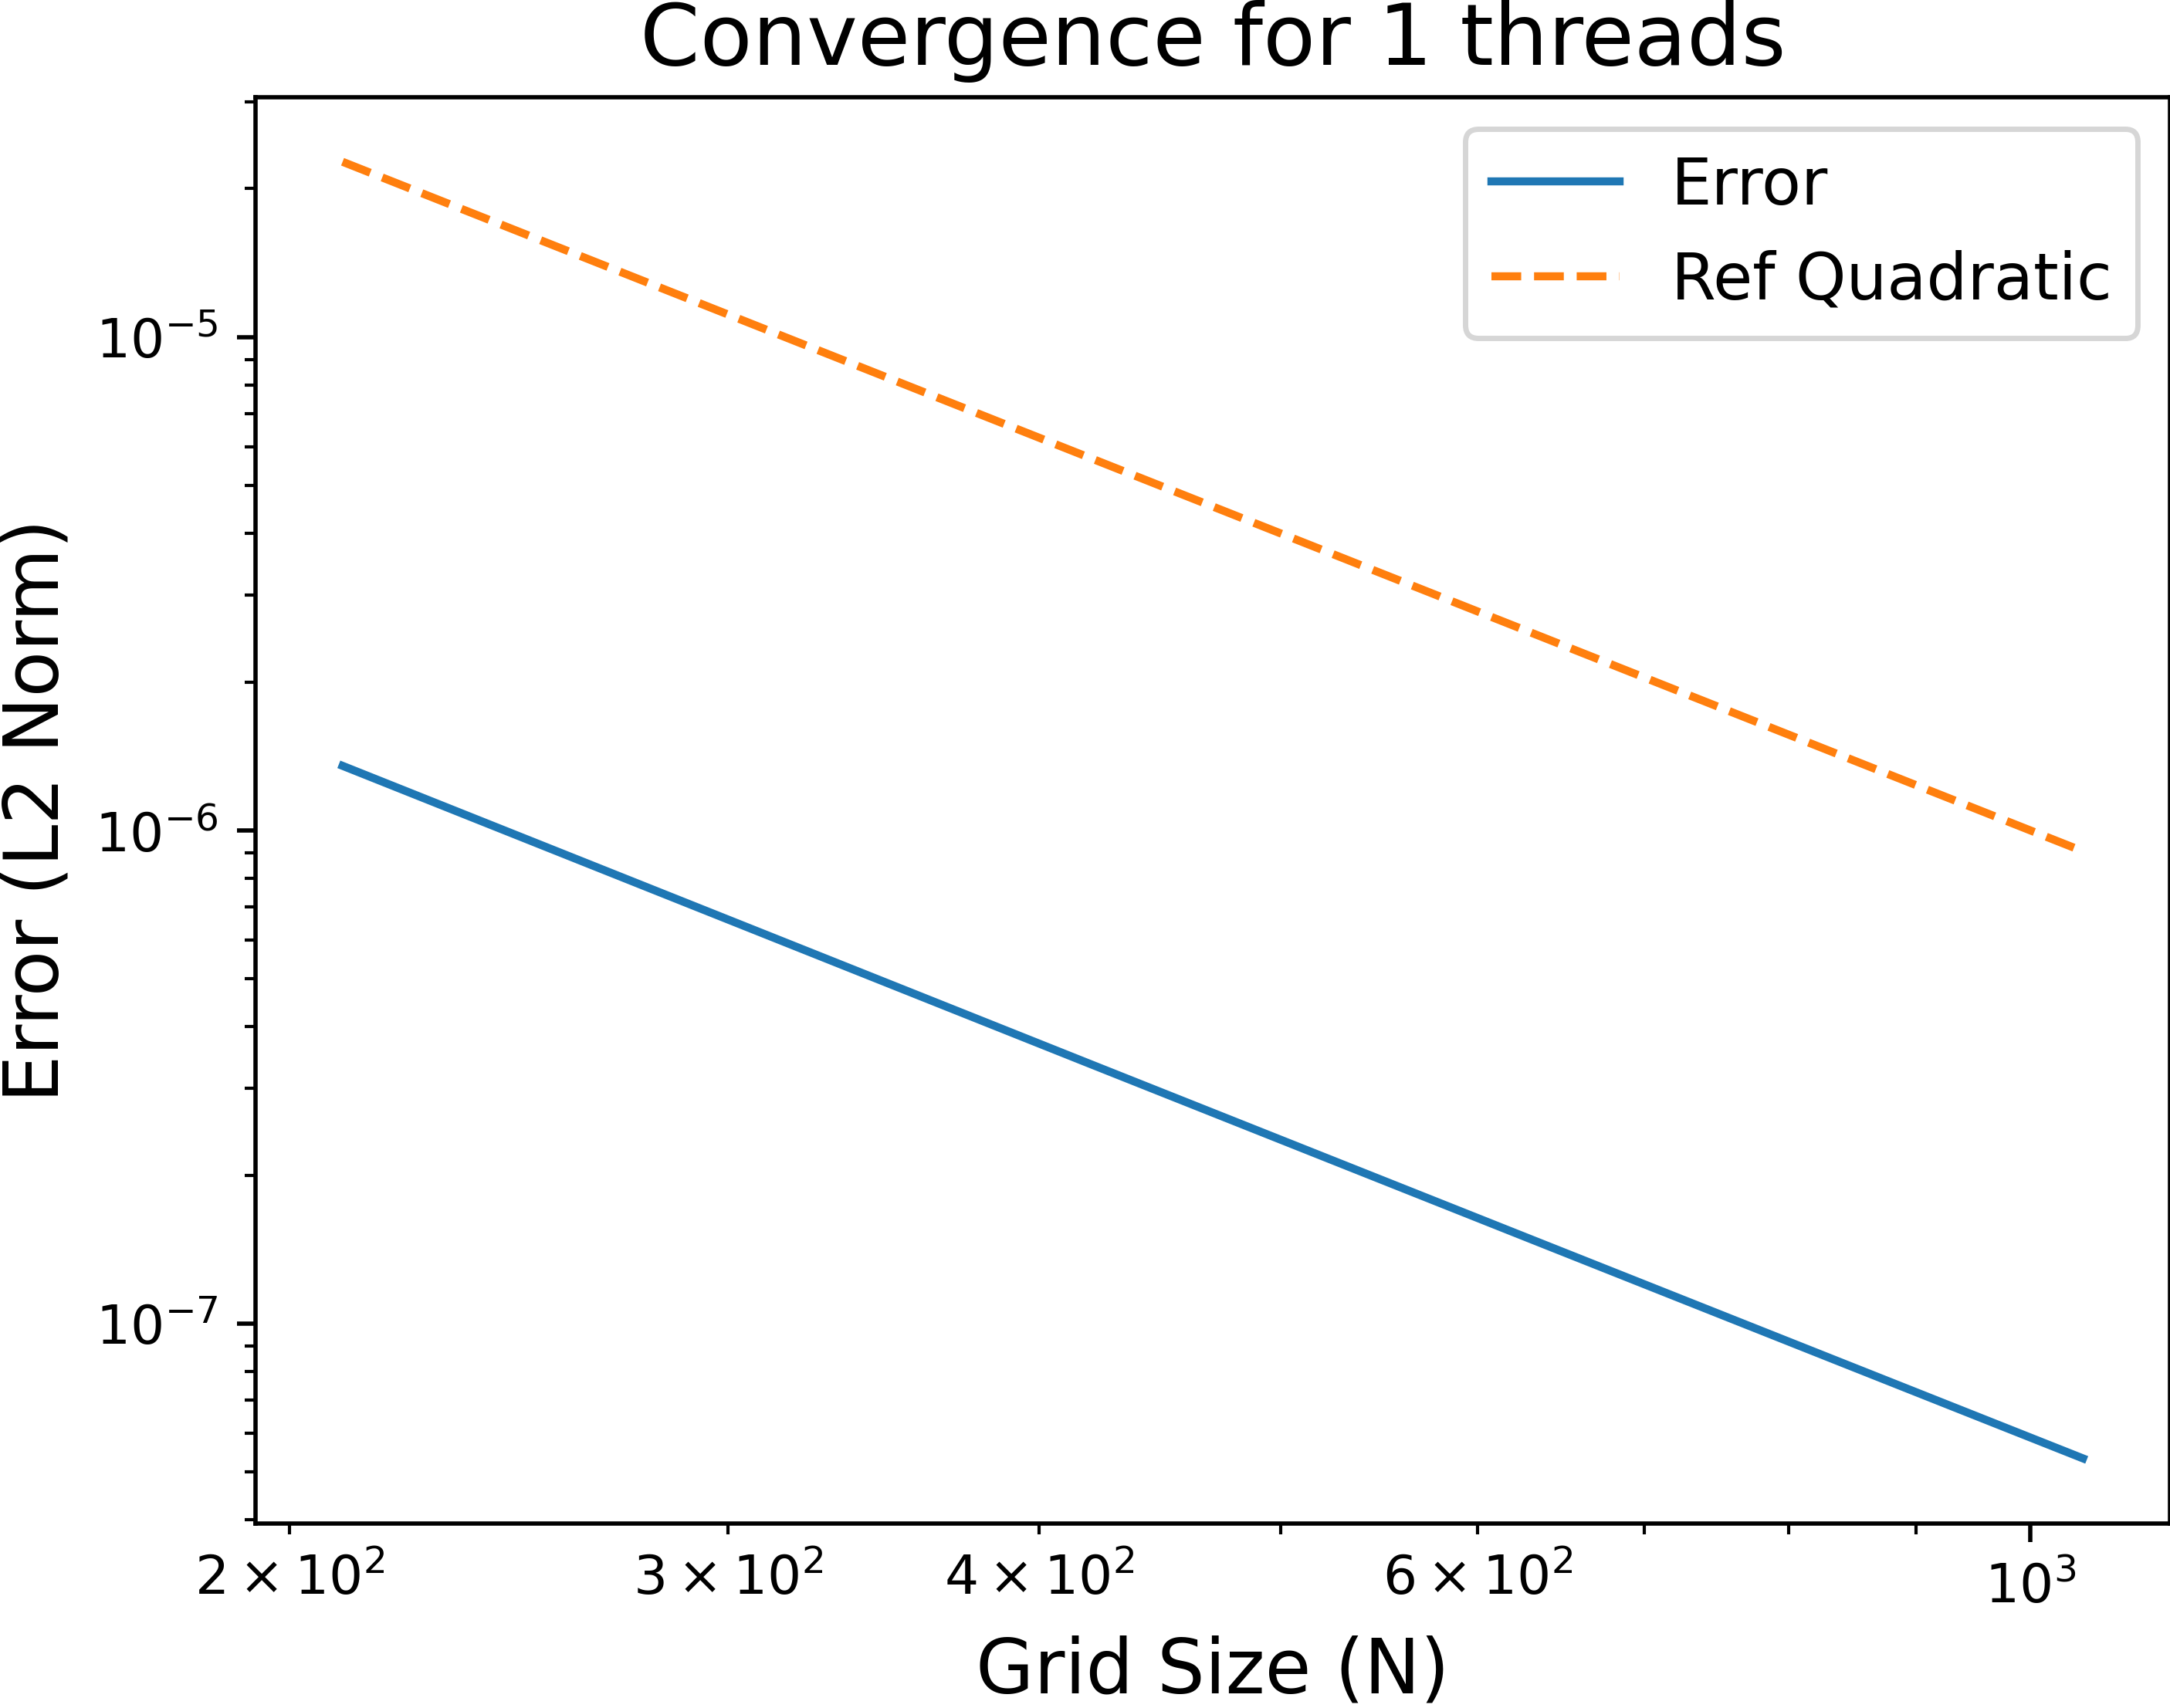
\includegraphics[width=0.5\textwidth]{/Users/stevenzuniga/Desktop/HPC/finite-difference-threading/report/error_1threadLocal.png}
\caption{Error plot for 1-thread computation.}
\label{fig:error_1threads}
\end{figure}

%2-thread
\begin{figure}[H]
\centering
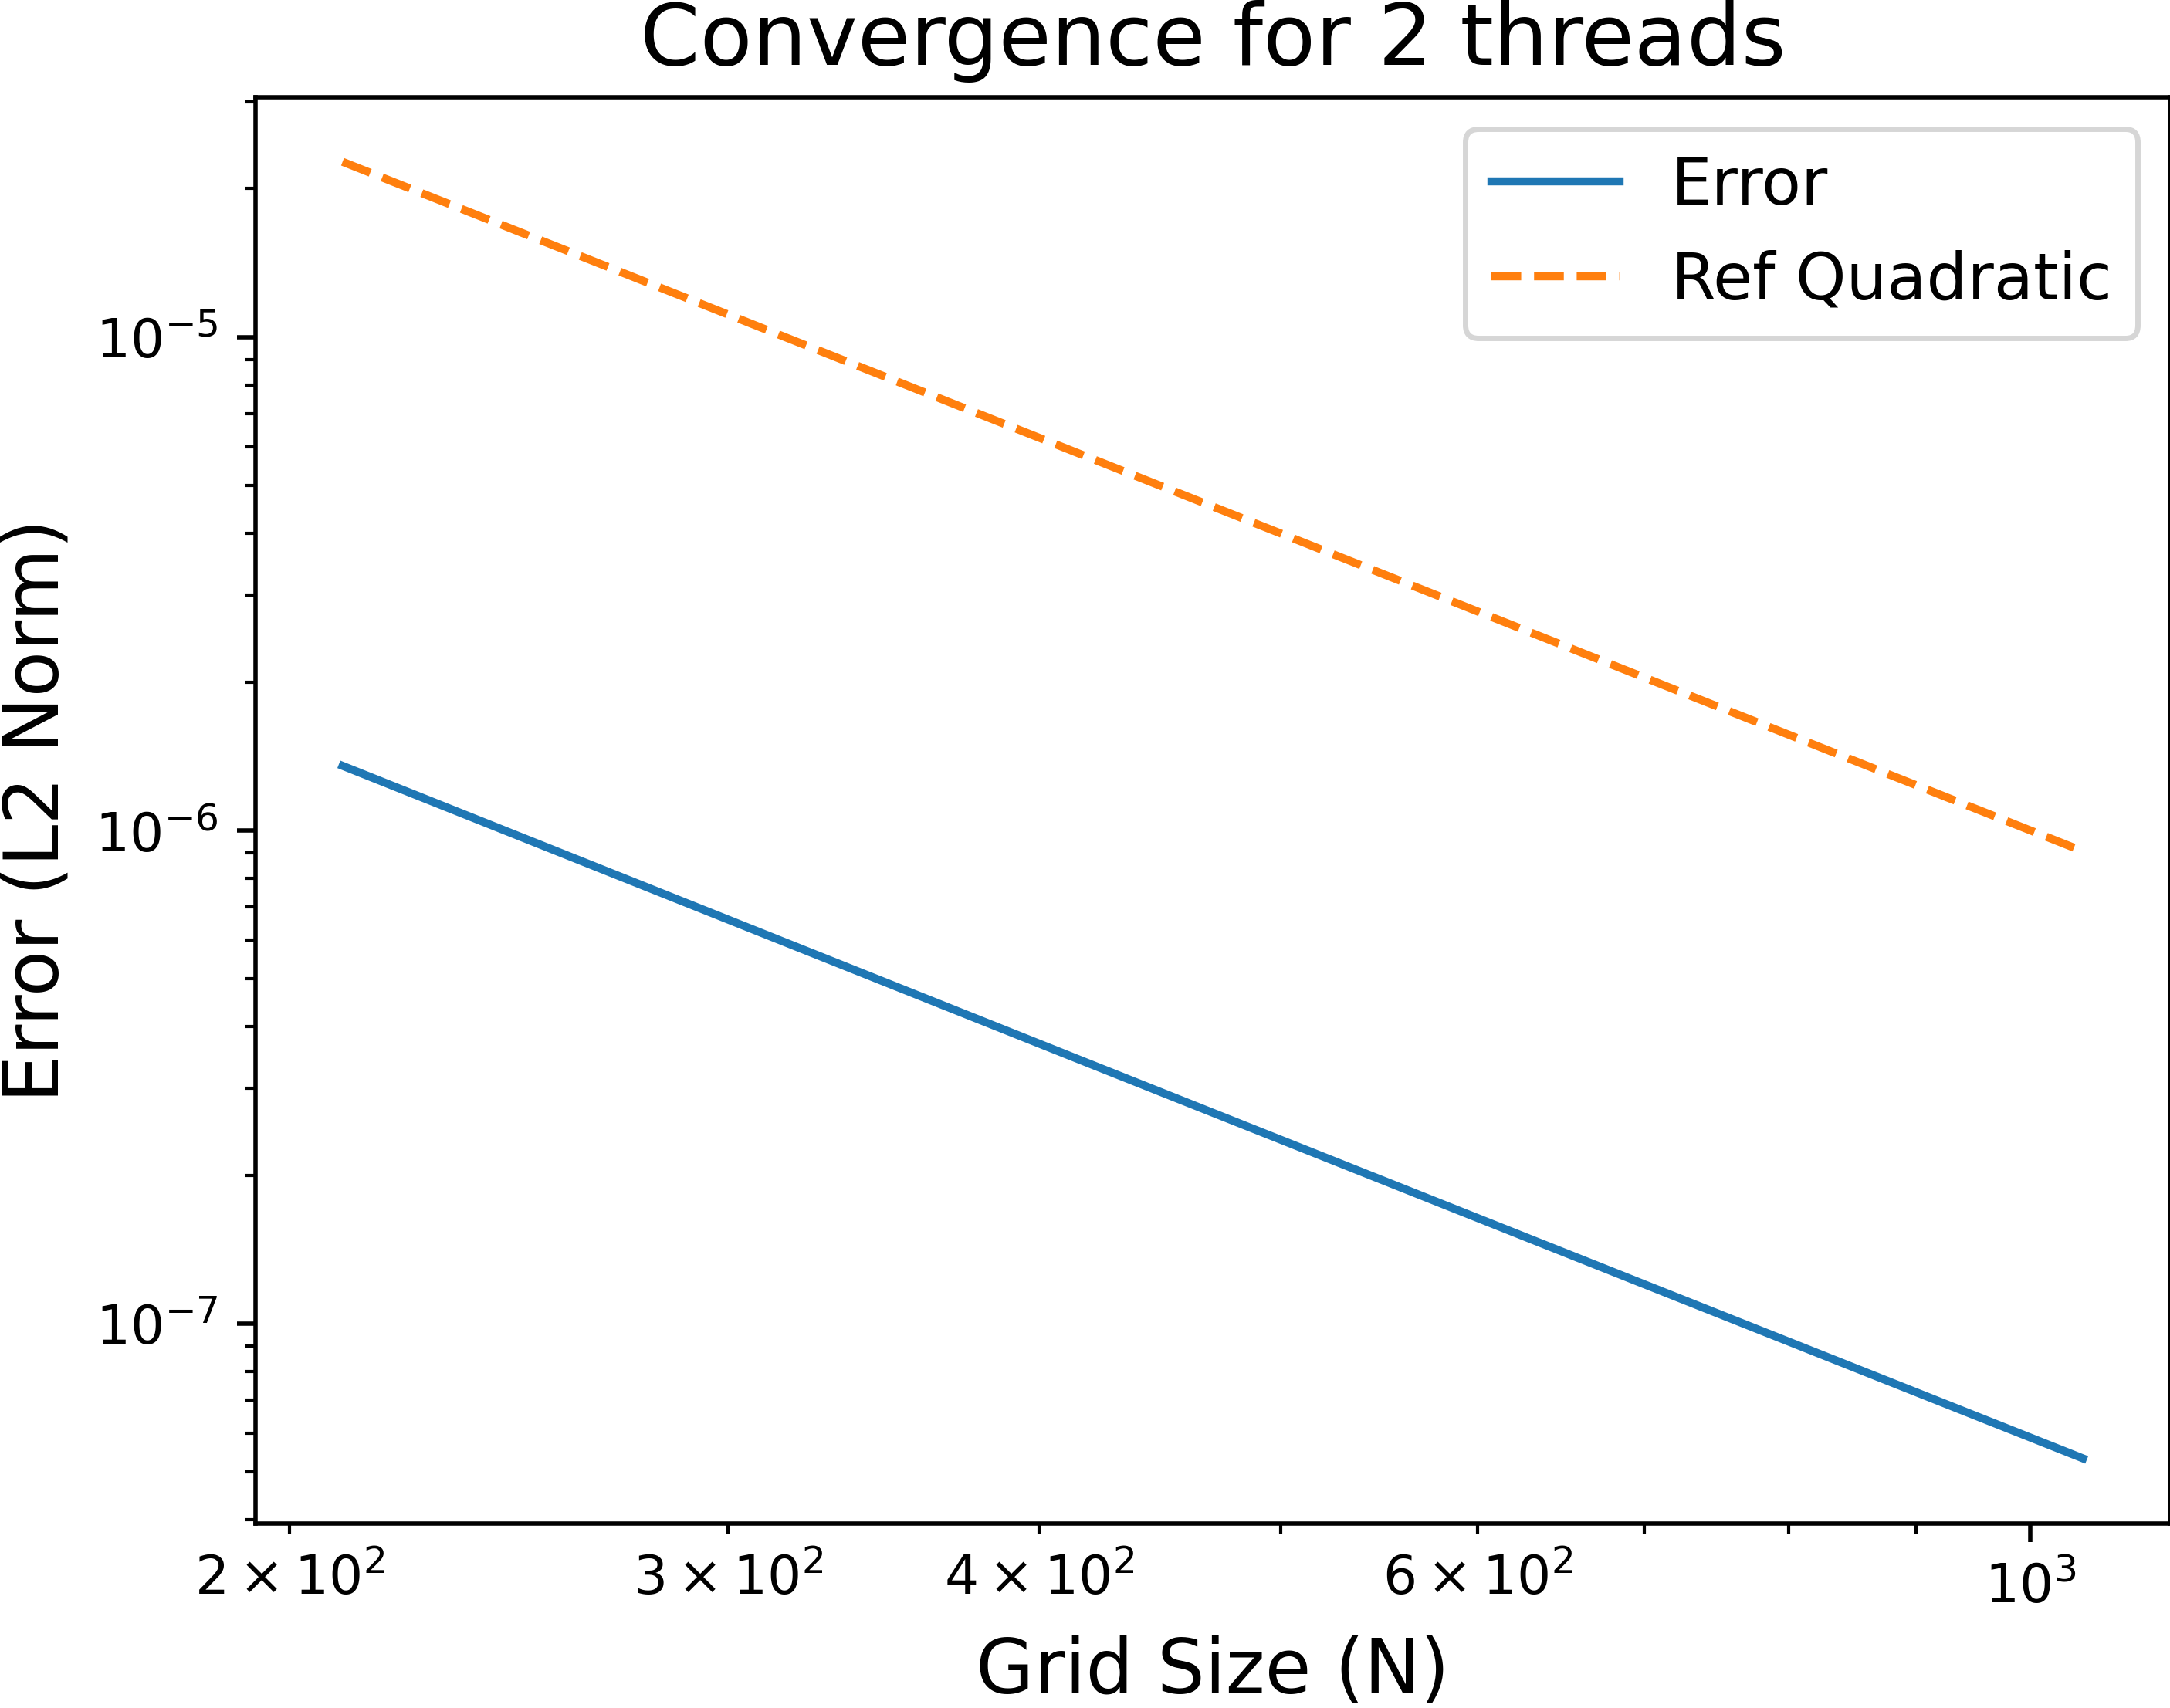
\includegraphics[width=0.5\textwidth]{/Users/stevenzuniga/Desktop/HPC/finite-difference-threading/report/error_2threadLocal.png}
\caption{Error plot for 2-thread computation.}
\label{fig:error_2threads}
\end{figure}

%3-thread
\begin{figure}[H]
\centering
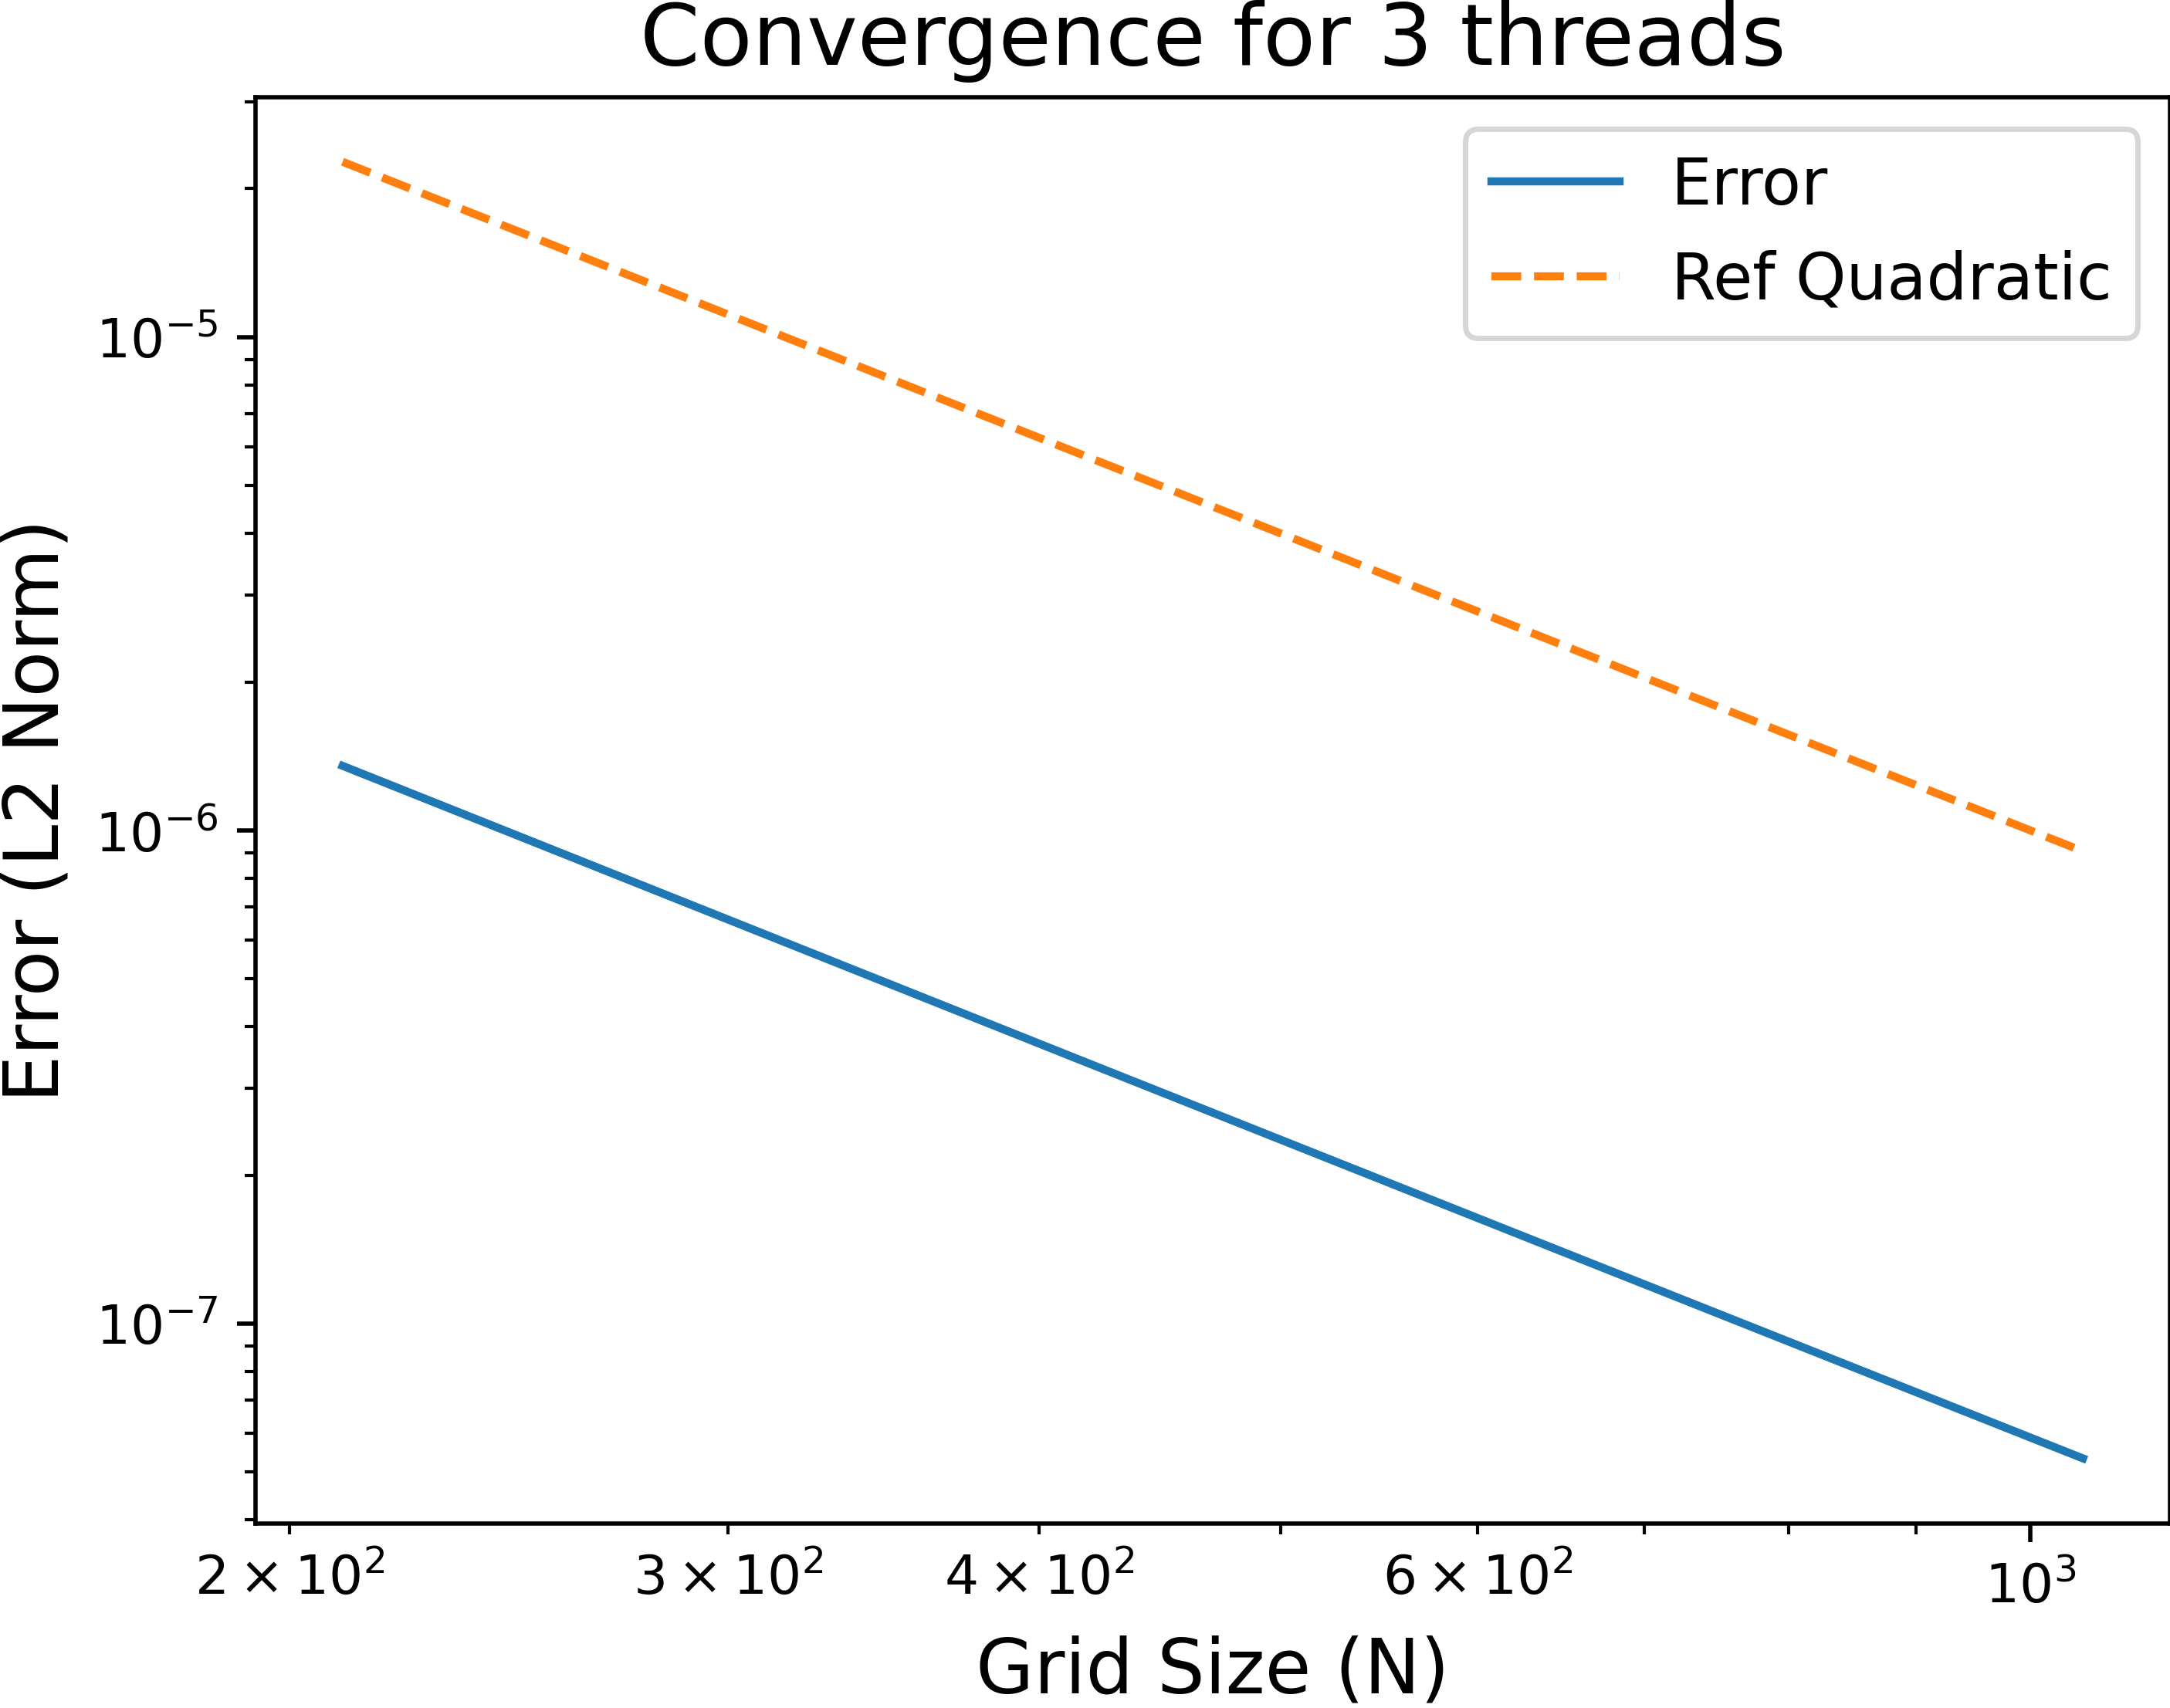
\includegraphics[width=0.5\textwidth]{/Users/stevenzuniga/Desktop/HPC/finite-difference-threading/report/error_3threadLocal.png}
\caption{Error plot for 3-thread computation.}
\label{fig:error_3threads}
\end{figure}

These error plots confirm that our numerical method achieves the expected quadratic convergence as \( h \rightarrow 0 \). This behavior aligns with the theoretical performance of the second-order finite difference scheme, demonstrating the accuracy of our implementation.

Each thread was assigned a 1D domain partition with "halo" regions to ensure accurate computation at boundaries shared with neighboring threads. This approach helped in distributing the computation load evenly across threads. Each thread handled \(\frac{n}{\text{nt}}\) rows. Halo regions allowed threads to access neighboring data for finite difference calculations.

\subsection{CARC Performance Analysis}
To understand the scalability and performance of the parallel implementation, we conducted strong scaling studies on the CARC supercomputing platform. This analysis involved running the parallel code on a single CARC node using problem sizes specified by option “2” in the homework skeleton.

\subsubsection{Parallel Efficiency}
Parallel efficiency was calculated using the formula:
\[
E_p = \frac{T_1}{T_p \cdot p},
\]
where \( T_1 \) is the execution time for the serial code, \( T_p \) is the execution time for the parallel code using \( p \) threads, and \( p \) is the number of threads. 

Figure \ref{fig:efficiency_threads} shows the parallel efficiency as the number of threads increased. The efficiency remained high for lower thread counts but gradually decreased as more threads were used. This behavior indicates that, while parallelization significantly reduced computation time, the benefits of adding more threads beyond a certain point were constrained by factors such as data synchronization and the halo region data transfer between threads.

\begin{figure}[h!]
\centering
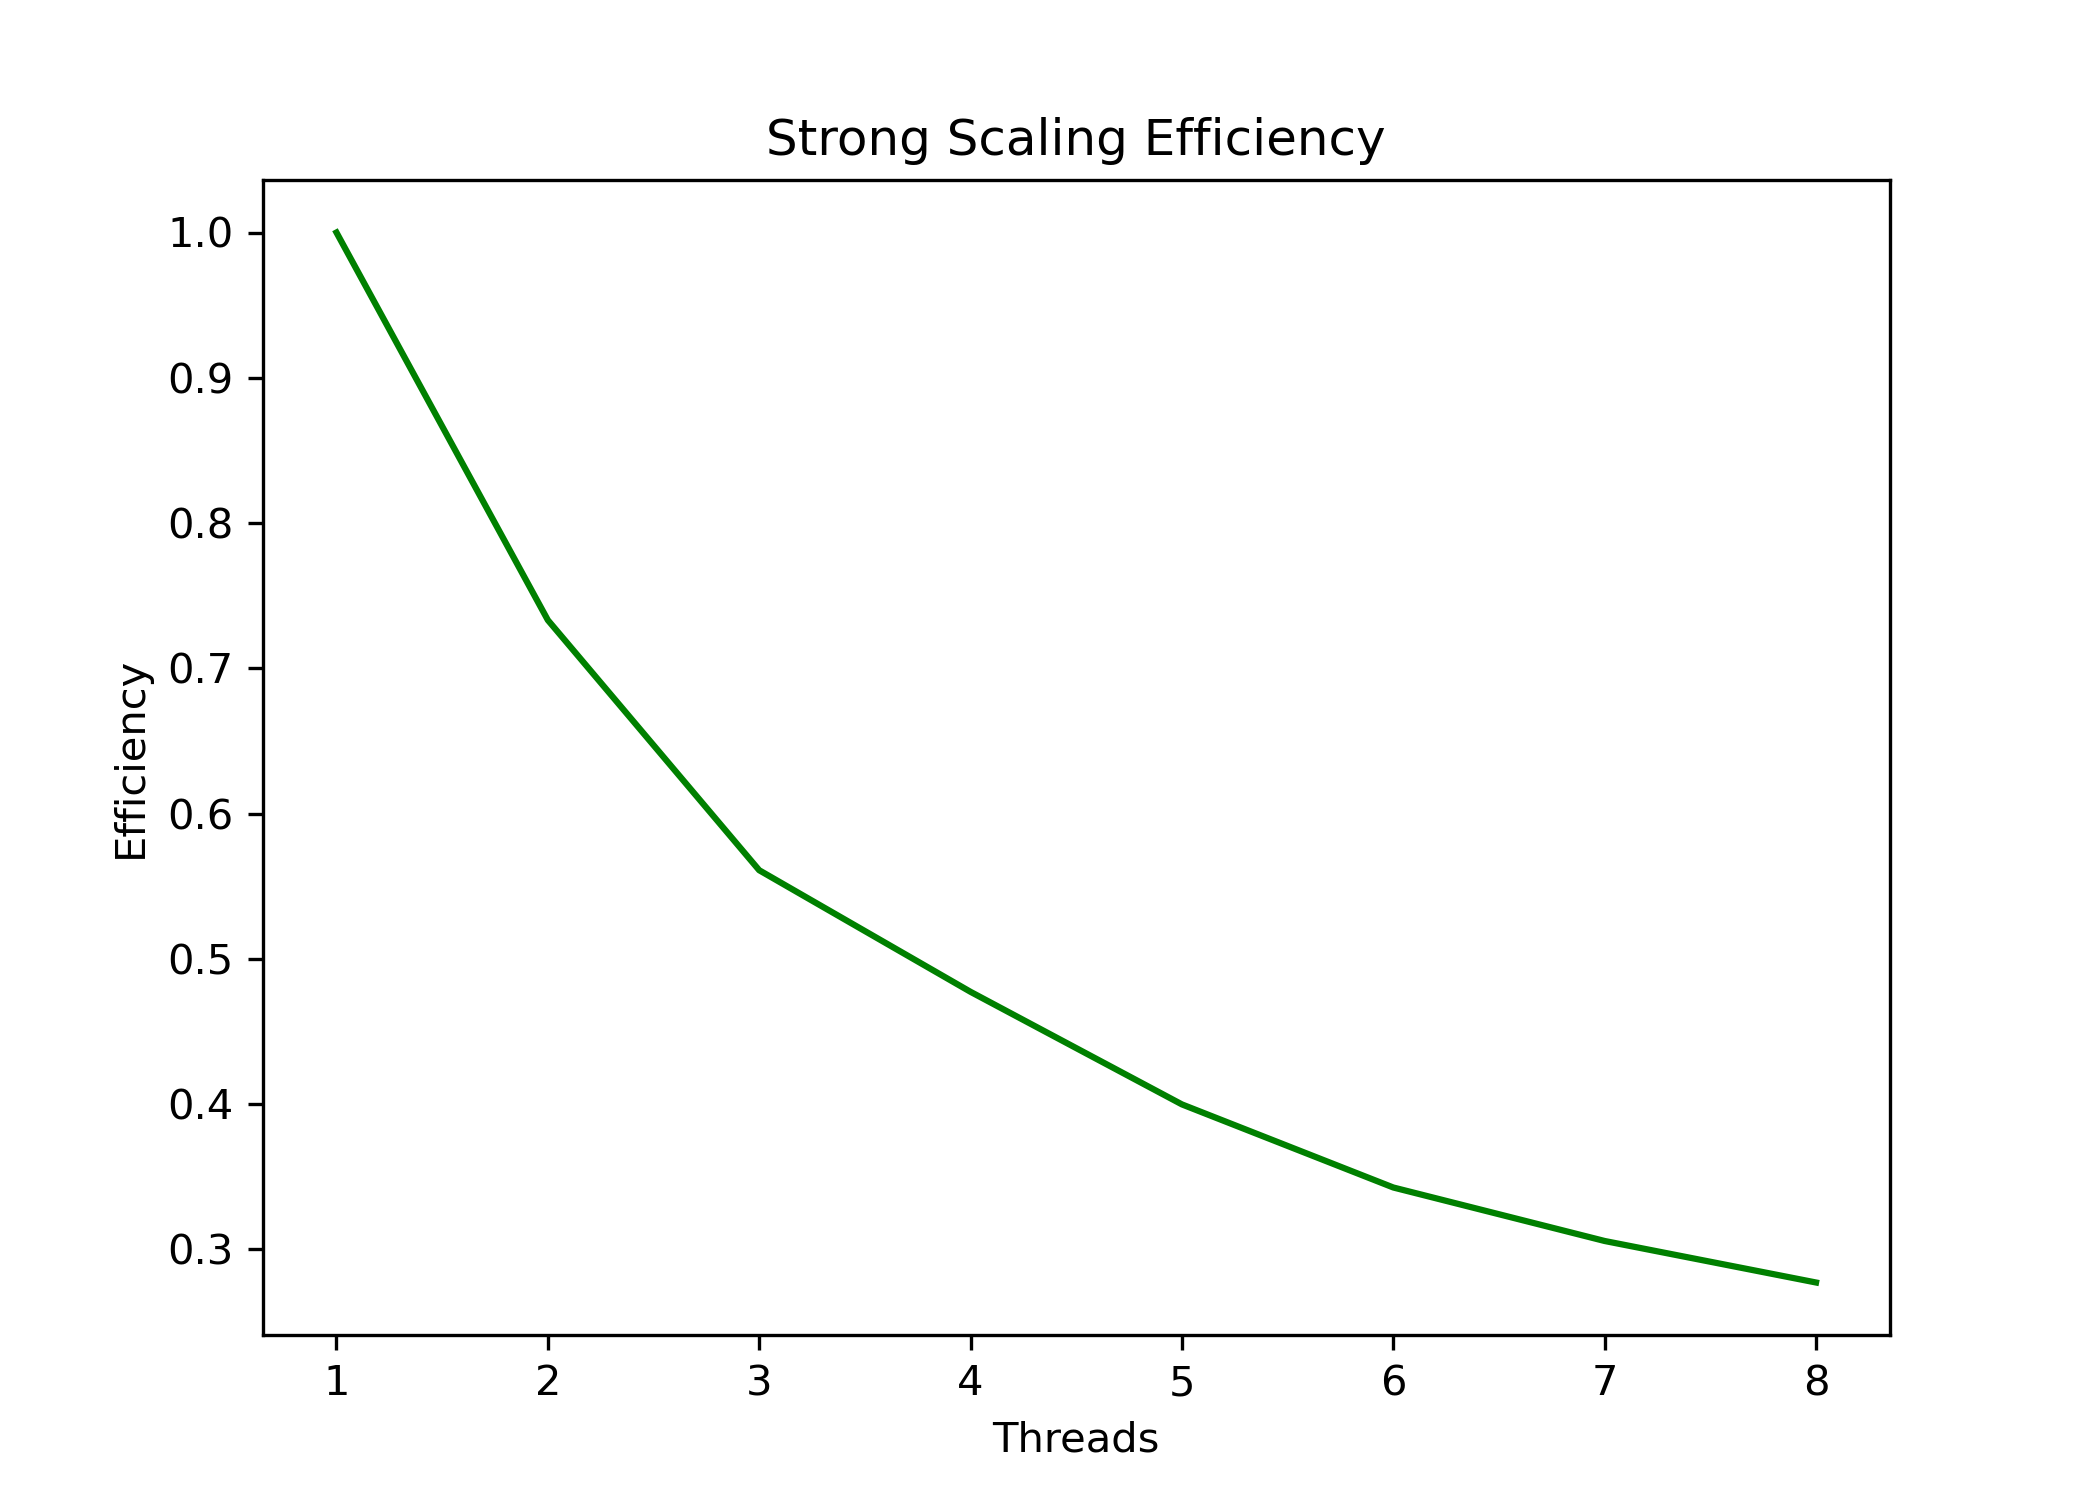
\includegraphics[width=0.5\textwidth]{/Users/stevenzuniga/Desktop/HPC/finite-difference-threading/report/efficiency_vs_threads.png}
\caption{Parallel efficiency vs. number of threads.}
\label{fig:efficiency_threads}
\end{figure}

\FloatBarrier
\subsubsection{Execution Time}
Figure \ref{fig:time_threads} illustrates the execution time for different numbers of threads on CARC. The execution time decreased as the number of threads increased, showing improved performance due to parallel computation. This trend confirms that CARC's multi-core architecture effectively distributes the workload and reduces overall computation time. However, diminishing returns were observed as more threads were utilized, suggesting that synchronization and communication overheads limited further speedups.

\begin{figure}[h!]
\centering
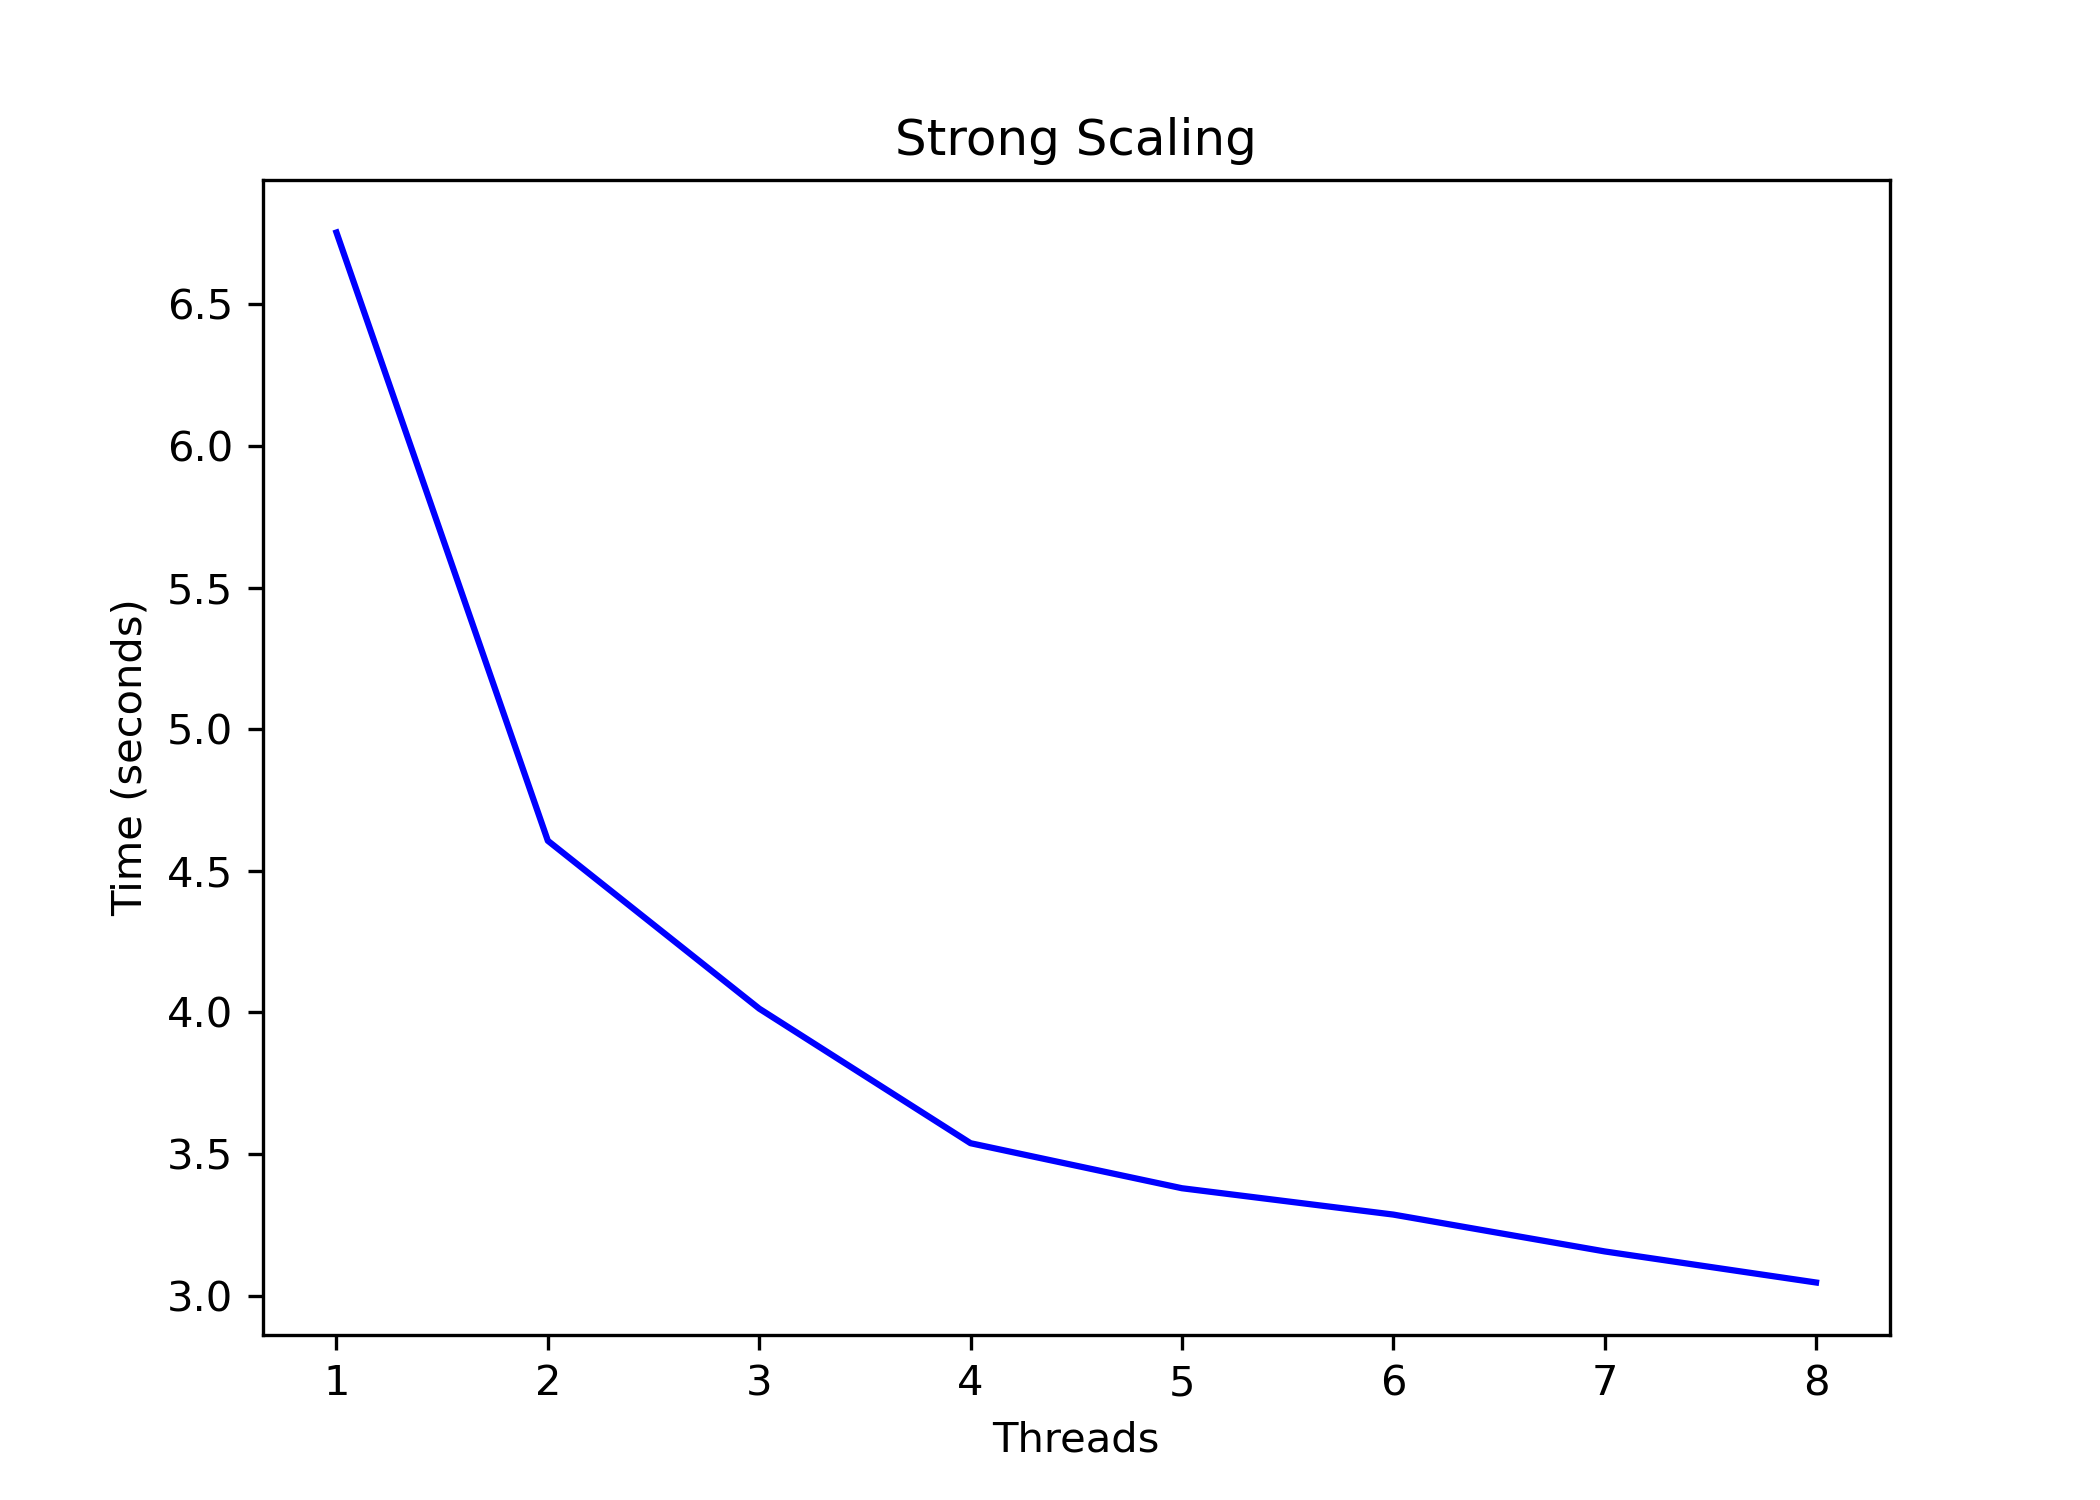
\includegraphics[width=0.5\textwidth]{/Users/stevenzuniga/Desktop/HPC/finite-difference-threading/report/time_vs_threads.png}
\caption{Execution time vs. number of threads.}
\label{fig:time_threads}
\end{figure}

\FloatBarrier

\section{Conclusion}
The CARC performance analysis revealed:\\

Strong Scaling Performance: The implementation demonstrated strong scaling up to a moderate number of threads, aligning with theoretical expectations for parallel finite difference computations.

Overhead Analysis: As the number of threads increased, the communication overhead associated with managing halo regions and synchronization became more pronounced. This resulted in a plateau in performance improvements.

Optimal Thread Count: The results suggest that an optimal number of threads exists beyond which adding more threads does not yield significant performance benefits. This threshold is a function of the problem size and the computational complexity of managing shared data.

The use of the CARC platform allowed for uniform results and greater computational resources, which would not have been possible on a local machine. This analysis highlights the importance of understanding the limitations of parallel programming, including overhead and memory bandwidth constraints, in large-scale scientific computing.











\end{document}
